\section{Background \& related work}
\todo[inline]{%
    \textcite{satyanarayanan2009case}

    Other papers detailing the advantages of Edge computing.

    Next, what applications benefit from the Edge?
    \gls{WCA}! Mention both the main body of work (by Satya et.\ al.) but also other authors out there.
    Main points: prototypes and characterization of system latencies and load.
}

\subsection{Edge computing}

Edge computing is a novel distributed computing paradigm, emerging from a need to overcome the drawbacks of offloading computation and data to the cloud.
Cloud computing, the reigning distributed computing model, allows users to access shared pools of resources such as servers, databases, and applications, over the internet~\cite{gai2012towards}.
These pools of resources are managed in a centralized manner by specialized providers, and users and businesses can access them on-demand, without having to invest in and manage infrastructure of their own.
Providers in turn employ economies of scale, providing these services by deploying massive amounts of computing power and storage capacity in specialized locations known as datacenters~\citationeeded.
These hardware resources are then further compartmentalized through the use of virtualization technologies such as \glspl{VM} and containers~\cite{gai2012towards}.

Through this design, cloud computing affords significant advantages to users.
As services are deployed in a centralized manner accessible over the internet, users can interact with their data and applications from anywhere in the world, from any device.
Thanks to economies of scale and virtualization technologies, the cloud is highly scalable;
services can be scaled simply by spawning more \glspl{VM}.
The specialized nature of cloud providers, the scale of modern datacenters, and the use of virtualization also make the cloud highly reliable.
When hardware fails, recovering is simply a matter of migrating the service container or \gls{VM} to an available compute node~\cite{endo2016high}.

However, the cloud is not suitable for everything, and presents important drawbacks and challenges for latency-sensitive applications.
In order to achieve the necessary economies of scale, cloud datacenters are designed to serve users distributed across vast geographical areas.
These installations are thus often located ``far'' from potential users;
for instance, at the time of writing, \gls{AWS} processes traffic from all of Scandinavia and the Baltic countries through a single datacenter in Stockholm~\cite{awsregions}.
This leads to prohibitively high latencies for both highly interactive immersive applications such as mobile \gls{XR} and for \glspl{CPS} and \glspl{NCS}~\cite{satyanarayanan2009case,varghese2016challenges,shi2016promise}.
The former category requires \emph{motion-to-photon} latencies (i.e.\ time between input capture and feedback) below \SI{60}{\milli\second} for interactions to be perceived as fluid and responsive by the user~\cite{chen2017empirical}; the latter can require sub-\SI{10}{\milli\second} latencies, for instance in the case of vehicular safety systems.
Such latencies are unfeasible to consistently achieve with cloud computing~\cite{dang2021cloudy}.

Current cloud infrastructures are also ill-suited to deal with the bandwidth requirements of the \gls{IOT} and of mobile computing.
As smart devices, appliances, and sensors become more and more ubiquitous, the network architectures of modern datacenters face significant challenges to deal with the massively increasing volume of traffic~\cite{shi2016edge,wang2019towards}.

\begin{figure}
    \centering
    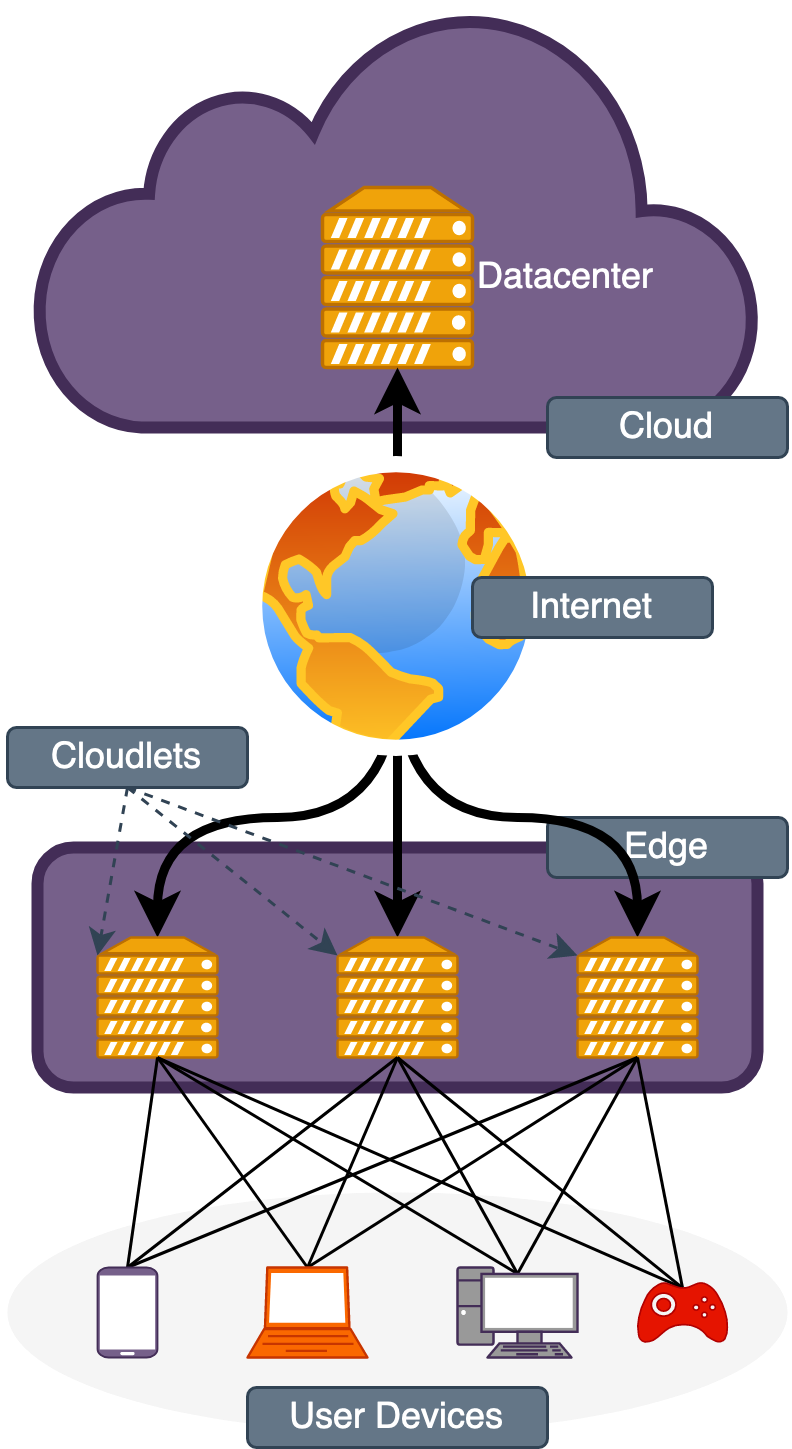
\includegraphics[height=30em]{Figs/edgecomputing}
    \caption{%
        Conceptual design of edge computing.
        Micro-clouds (known as ``cloudlets''~\cite{satyanarayanan2009case}) are placed a at the edge of the network, a few hops away from end users.
        In other words, these cloudlets are located between users and the internet and the cloud.
    }\label{fig:edgecomputing}
\end{figure}

Edge computing, emerges as a potential answer to these challenges~\cite{satyanarayanan2009case,shi2016promise,shi2016edge,varghese2016challenges,satyanarayanan2017emergence,wang2019towards}.
This term refers to a novel distributed computing paradigm, complementary to cloud computing, which tackles the challenges of the cloud by moving computation closer to where it is needed.
Instead of offloading computation to a datacenter potentially thousands of kilometers away, in edge computing it is offloaded to a micro-datacenter --- a \emph{cloudlet}~\cite{satyanarayanan2009case} --- at the \emph{edge} of the network.
These coudlets feature most of the key characteristics of cloud datacenters, such as multi-tenancy, virtualization of computing resources, virtually unrestricted access to energy, as well as limited scalability, one or two hops away from the user (see \cref{fig:edgecomputing})

The architecture of edge computing offers several advantages.
Thanks to their proximity to users, cloudlets can serve highly latency-sensitive and resource-intensive applications with extremely low latencies while still providing orders of magnitude more computing and energy resources than those present on mobile and wearable devices.
Mobile \gls{XR}, such as \gls{WCA}~\cite{ha2014towards,chen2018application,wang2020scaling,chen2017empirical,chen2018application}, and 5G-enabled \glspl{CPS} and \glspl{NCS}~\cite{sasaki2016vehicle,wang2018bandwidth,wan2020efficient} are uniquely poised to take advantage of this characteristic of edge computing.


\subsection{\glsfmtshort{WCA} and other \glsfmtshort{XR} applications}

There is increasing interest from academia and industry in novel applications such as immersive \gls{AR} or \gls{WCA}~\cite{chatzopoulos2017hyperion,ha2014towards}, also known as human-in-the-loop applications.
These applications aim to seamlessly integrate into the lives of users to provide real-time, context-aware information by capturing user and environment information and leveraging compute-intensive algorithms to analyze the data in order to provide real-time feedback to the user.
Sensory input, such as video, audio, and other user-related data such as orientation and movement, are examples of what is typically captured, while the backend generally employs machine learning technologies such as \glspl{DNN}~\cite{ha2014towards}.
\Cref{paper:olguinmunoz2019edgedroid:fig:pipeline2} depicts such a system.
These applications are highly latency sensitive, measuring latency as the time from the capture of the sensory information until feedback is received.
Delays above a certain threshold can hurt the user experience or even make the application unusable~\cite{chen2017empirical}.

In literature, these challenging latency requirements have so far mainly been addressed through research on the optimal placement of the compute process.
There is a broad understanding today that with the advent of edge computing, human-in-the-loop applications will become viable~\cite{bittmann2017edge,flinn2012cyber,chen2017empirical,ha2013just}.
However, with respect to end-to-end latency, there are many more trade-offs involved than merely the question of where the compute backend is placed.
A human-in-the-loop application consists of various processing steps that can be influenced during the development of the application.
What kind of compression to apply to the sensory input on the uplink; which backend algorithms to utilize; how to stage the backend; when to send feedback to the human users; and how to manage congestion on the loop, as well as wireless channel fluctuations --- all these design choices impact the latency of the application.
There are also many design choices in the infrastructure: how is the sensory input conveyed to the point of computation (i.e.\ by which wireless system; with which transmission/prioritization scheme); which hardware is running at the backend; which operating system; how is the feedback conveyed back to the human user?
Finally, in production use these applications will most likely run concurrently with others.
How does this, together with other best-effort applications, impact the latencies perceived by the human user?
Existing studies~\cite{ha2014towards,chen2015early,satyanarayanan2009case,chatzopoulos2017hyperion} of this class of applications have only lightly touched upon these issues~\cite{chen2017empirical}.
On the other hand, recently published models for end-to-end latency of edge computing architectures~\cite{al_zubaidy2015performance,schiessl2017finite} are quite complex, while not accounting for the specifics of human-in-the-loop applications.
We only have a coarse understanding of the many degrees of freedom upon which end-to-end latency depends.

The goal of this paper is to provide a methodological approach to studying these latency trade-offs, along with a tool, EdgeDroid 1.0\footnote{We plan to make the EdgeDroid 1.0 benchmarking suite available as Free and Open Source Software and the recorded traces under a Creative Commons License.}, that simplifies the benchmarking of human-in-the-loop applications.
We view EdgeDroid 1.0 to be the very first, and simplest, of a family of tools that will embody increasingly sophisticated and accurate models of user behavior.

Wearable Cognitive Assistants, \gls{WCA} for short, have recently started to garner attention from the research community~\cite{ha2014towards,chen2015early}.
They represent a novel category of highly interactive and context-sensitive augmented reality applications, that aim to amplify human cognition in both day-to-day tasks and professional settings.
Their mode of operation is analogous to how \gls{GPS} navigation systems guide drivers, by seamlessly providing relevant instructions and feedback relating to the current task at hand.
Note that this implies seamless interaction with the context of the user --- at no moment does the user need to trigger an update explicitly, as the application is constantly tracking the state of the target task.
An example is an IKEA Assistant~\cite{IKEAAssistant} which monitors the assembly of a piece of furniture in real time, providing timely, step-by-step feedback to guide the user toward completion.

WCA systems were originally inspired by assistive use cases for people suffering from some form of cognitive decline, either through aging or because of traumatic brain injuries~\cite{ha2014towards,satyanarayanan2019augmenting}.
More recently, they have been applied to a broader range of use cases, including step-by-step guidance on complex assembly tasks~\cite{chen2017empirical}.
Non-wearable augmented reality and cognitive assistance systems have already been proven to be valuable tools in the industrial workplace~\cite{funk2015cognitive,gorecky2011cognito}.
Detethering this assistance from its current fixed location will surely make it available to many more fields.

Based on these use cases, we identify three main requirements for \gls{WCA}:\@
\begin{enumerate}
    \item \gls{WCA} systems should be available whenever the user requires them, without being tethered to a particular physical location. Assistants need to be pervasive and mobile.

    \item Interaction with the system should be immersive and seamless, i.e.\ the assistant should be able to analyze the current context and automatically provide relevant feedback without explicit commands from the user.
    In this sense, \gls{WCA} is expected to operate much like a human assistant would, by observing the performance of the user and offering guidance proactively.

    \item Feedback should be ``quick'', relative to the task at hand.
    This requirement is further strengthened by the previously mentioned ``seamless interaction'' characteristic of these systems.
    This means that users will have expectations of constant, immediate feedback as they progress through the task.
    In the case of a step-by-step task like IKEA, delayed feedback might simply confuse or distract the user.
    However, in a highly interactive task like a \emph{Ping-Pong assistant}~\cite{PingPongAssistant,chen2015early} late guidance is at best a nuisance and at worst a severe handicap.
\end{enumerate}

\cref{paper:olguinmunoz2021impact:item:pervasive} implies use of lightweight and low-power devices, preferably a wearable device that frees both hands for work.
\cref{paper:olguinmunoz2021impact:item:interaction}, on the other hand, suggests a level of context sensitivity and proactivity that can only be provided by real-time analysis of sensor inputs such as video and audio feeds.
The compute-intensive processing suggested by \cref{paper:olguinmunoz2021impact:item:interaction} cannot be met by the lightweight wearable devices suggested by \cref{paper:olguinmunoz2021impact:item:pervasive}.
Only by offloading computation from a wearable device to cloud-based or edge-based infrastructure can this circle be squared.
However, offloading implies an extended end-to-end pipeline with many potential sources of queueing, transmission, and processing delays.
\cref{paper:olguinmunoz2021impact:item:lowlatency} therefore emerges as a key concern, requiring deep understanding of the impact of end-to-end delays on \gls{WCA} users.

% However, additional challenges remain in the path toward widespread adoption.
\cref{paper:olguinmunoz2021impact:item:lowlatency} forms the base motivation for the research presented in this paper.
We still have a very limited understanding of how humans react to delays in these systems --- specifically, how changes in system responsiveness impact users.
\emph{System responsiveness} here denotes a qualitative scale ranging from \emph{high} (that is, not subject to delay or subject to negligible delay with respect to human perception) to \emph{low} (i.e.\ subject to considerable delay).
% Conversely, QoE is understood to range from \emph{good} (i.e.\ users enjoy interacting with the application) to bad (users dislike interacting with the application).
Characterizing the relationships between system responsiveness and user behavior and quality of experience is of paramount importance for the design and evaluation of these applications.
It is generally acknowledged, for instance, that a system going from a state of high responsiveness to one of low responsiveness can cause a drop in quality of experience~\cite{dabrowski201140}.
Furthermore, this could cause users to modify the temporal paramaters of their behavior when interacting with the system, generating a sort of \emph{feedback loop} between user and system.
A clear understanding of these relationships would allow, for instance, for the development of strategies for load balancing and optimization for large-scale deployment of \gls{WCA}.\@

\begin{figure}
    \centering
    \begin{subfigure}{\columnwidth}
        \centering
        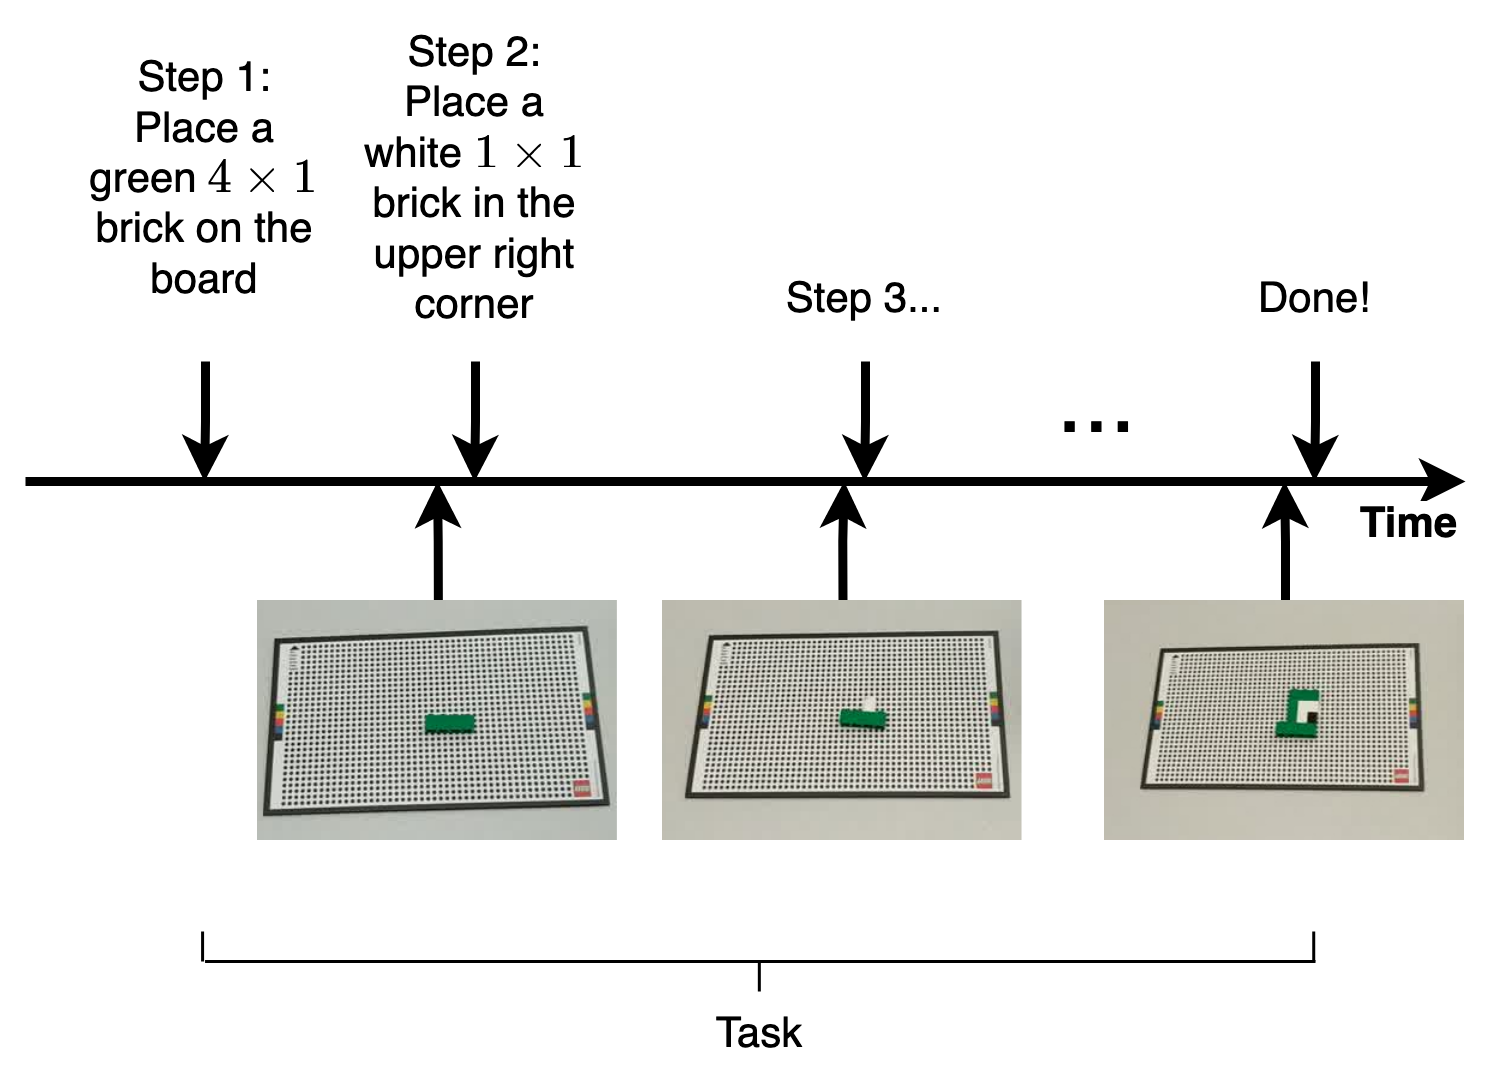
\includegraphics[width=\columnwidth]{publications/2023EdgeDroid2/figs/task.png}
        \caption{%
            Overview of a task in a \gls{WCA}, composed of a series of steps.
            Each steps starts with an instruction being provided to the user and ends with the instruction for the next step.
            The \gls{WCA} continuously samples the task state, automatically triggering transitions between steps as correct (or incorrect) states are recognized.
        }\label{background:fig:wcatask}
    \end{subfigure}\\
    \begin{subfigure}{\columnwidth}
        \centering
        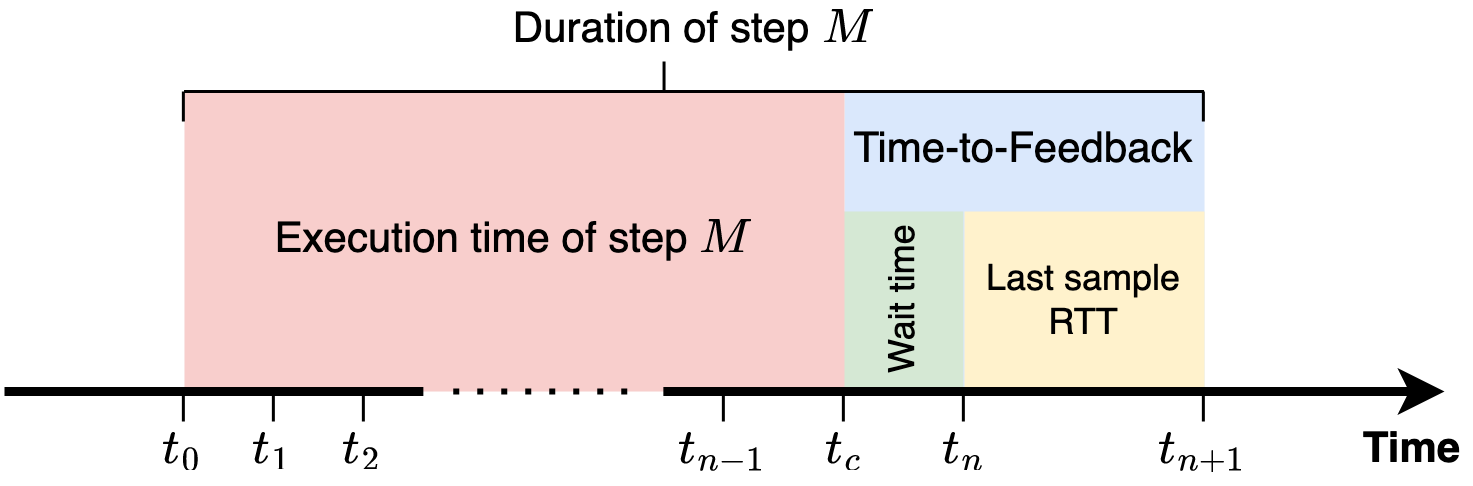
\includegraphics[width=\columnwidth]{publications/2023EdgeDroid2/figs/step_time.png}
        \caption{%
            Breakdown of a step into its timing components.
            The instruction for step \( M \) and \( M + 1 \) are provided to the user at \( t_0 \) and \( t_{n+1} \), respectively.
            \( t_k | k \in \{1, \ldots, n \} \) correspond to the \gls{WCA} sampling instants for step \( M \), and \( t_c \) marks the instant at which the user finishes performing the instruction.
        }\label{background:fig:wcastep}
    \end{subfigure}
    \caption{Key concepts in \gls{WCA}}
\end{figure}

\glspl{WCA} applications represent a category of novel, context-sensitive and highly-interactive \gls{AR} applications.
In this work we focus on a particular category --- ``step-based'' \gls{WCA} --- that have as their goal the guiding of a user through a sequential task.
Examples of such applications are the LEGO and IKEA assistants~\cite{Chen2015LEGO,Chen2018application}, in which users are guided step-by-step through the process of assembling a LEGO model and an IKEA lamp, respectively.

Step-based \glspl{WCA} operate analogously to how \gls{GPS} navigation assistants guide users, by seamlessly and continuously monitoring the progress of the user and autonomously providing relevant instructions and feedback.
The application follows the progress of the task in ``realtime'' by repeatedly sampling the state of the physical system, most commonly through video frames.
Whenever the assistant detects that the user has correctly or incorrectly performed an instruction, it provides a new instruction to either advance the task or correct the detected mistake.
The application otherwise remains silent and out-of-the-way of the user; that is, samples which do not generate a new instruction (e.g.~because they captured an intermediate or unfinished state, or simply noise) are silently discarded.
Herein lies one of the key characteristics of these applications: the user only consciously interacts with the application whenever they finish an instruction, and thus these are the \emph{only} points in time at which they can notice changes in system responsiveness.

In order to discuss these applications with precision we provide some definitions relating to their operation.
First of all, a \emph{step} is formally understood as a specific action to be performed by the user, described by a single instruction, and a \emph{task} consists of a series of steps to be executed in sequence (see \cref{background:fig:wcatask}).
A step begins when the corresponding instruction is provided to the user, and ends when the instruction for the next step is provided; we call the time interval between these two events the \emph{step duration}.

\glspl{WCA} employ sampling, most commonly of video feeds, to keep track of the state of the real world.
Take \( \{ t_0, t_1, \ldots, t_{n + 1} \} \) a series of discrete and sequential sampling instants at which the \gls{WCA} captures the state of the physical system, as illustrated in \cref{background:fig:wcastep}.
\( t_0 \) corresponds to the instant at which the instruction for step \( M \) is provided and the first sample is taken, and \( t_n \) to the instant at which the final sample (i.e.\ which captures the final state of step \( M \)) is taken.
\( t_{n + 1} \) is then the instant at which the result for sample \( t_n \) is returned and the instruction for step \( M + 1 \) is provided.
We define \( t_c \) as the point in time at which the user finishes performing the instruction for step \( M \), and the intervals \( t_c - t_0 \), \( t_n - t_c \), and \( t_{n + 1} - t_n \) as the \emph{execution time}, \emph{wait time}, and \emph{last sample \gls{RTT}}, respectively, of a step \( M \).
The sum of the latter two values (i.e.\ the interval \( t_{n + 1} - t_c \)) we call \emph{\gls{TTF}}, a metric which we will repeatedly refer to in this paper as it directly describes the responsiveness of a \gls{WCA}.

\subsection{Mechanisms relating human behavior to system responsiveness}

The question of how people respond to delay in a computer system is grounded in how people perceive time.
Time perception has been described as regulated by an attentional gate that, when opened, starts a cognitive pulse counter~\cite{zakay1995attentional,zakay1996role}.
More recent research indicates, however, that duration perception is highly malleable and the result of multiple timing mechanisms found in overlapping, flexible neural systems~\cite{bruno2016multiple,wiener2011multiple}.
The estimation of an event's duration varies with context of various types
\begin{enumerate*}[label={(\roman*)}, before=\unskip{: }, itemjoin={{; }}, itemjoin*={{; and }}]
\item events subsequent to a long or short interval are contracted or extended, respectively~\cite{heron2012duration}
\item repeated events tend to be perceived as shorter than novel ones~\cite{matthews2011stimulus}
\item arousal can expand durations~\cite{droit_volet2011emotion}.
\end{enumerate*}

Expectations play a critical role in time perception as well~\cite{zakay1995attentional,zakay1996role}.
It has been shown that people have a general tendency to be hypersensitive to delays in worse-than-expected states, and under-sensitive to meeting or exceeding expectations~\cite{loewenstein1992anomalies}.
Accordingly, failures to meet expected fast response times tend to be experienced as highly negative, whereas fast latencies are not noticed.
Violations of expectancy have a strong impact on the acceptability of computer systems.
Users of a computer system anticipate the latency for events, for which the standards only become more stringent as systems improve in response time.
In immersive systems like \gls{WCA}, which aim to provide seamless interaction, delays are particularly noticeable.

It has long been recognized that slow system response times can undermine cognitive processing, slow the pace of users, and lead to stereotyped behavior and errors, as well as cause negative emotional consequences~\cite{dabrowski201140}.
However, standards for what constitute tolerable delays have changed dramatically compared to three decades ago, when delays on the order of \SI{10}{\second} were deemed acceptable~\cite{nielsen1994usability, shneiderman2016designing, seow2008designing}.
Today's user context, and \gls{WCA} in particular, often demand response times orders of magnitude shorter.

For \gls{WCA} the acceptable range for latencies was explored by Chen et al.~\cite{chen2017empirical}, by constructing assistants for tasks with a range of time constraints, including step-by-step tasks and more interactive contexts like playing Ping-Pong against a human opponent.
They then proposed a latency tolerance zone according to the task demands.
For an essentially self-paced task like LEGO assembly, they found two key ranges of latency; unnoticeable, \SIrange{0}{0.6}{\second}; and impaired, \SIrange{0.6}{2.7}{\second}.
Beyond that, users could begin to show the negative outcomes previously catalogued~\cite{dabrowski201140}.

While behavioral changes and negative interaction outcomes have been well documented in prior research on system delay, the specific mechanisms that mediate these outcomes are less well understood.
These mechanisms could be cognitive or emotional in origin.

A first possible explanation comes from research on cognitive and motor planning.
Delay may move users from relatively automatic to more attention-demanding processing.
Cognitive and motor tasks are commonly described as a hierarchical system, progressing from high-level goals to the sequence of commands that accomplishes them.
As competency in a task increases, execution of the hierarchy becomes increasingly automated.
Automatization has been described from a computational perspective in {Anderson's ACT-R}~model as the compiling of multiple productions into one~\cite{neves1981knowledge}.
Neural measurements indicate that with automaticity, control moves from frontal brain areas to more posterior ones~\cite{jeon2015degree,puttemans2005changes}, and similar distinctions have been related to temporal processing~\cite{lewis2003distinct,koch2009neural,lee2019limiting}.

Although activities guided by a \gls{WCA} are not simple motor actions, immediate feedback after each of a series of repeated actions should promote development and automatic execution of a hierarchical plan.
Delays, in contrast, would disrupt such a plan through the loss of automated control~\cite{lee2019limiting}.

A second, alternative explanation of delay effects appeals to emotional systems rather than cognitive processes.
As users of a system become emotionally aroused by delay, they may be subject to generalized arousal, causing decrements in performance~\cite{lee2019limiting}.

Finally, a third potential explanation of delay effects is what has been called ``ego depletion'', the notion that expending effort on self-control eliminates resources needed for further effort~\cite{baumeister74tice,lin2020strong}.

The various processing accounts of delay effects predict different outcomes, which we will consider in the context of the current data.
If delay increases attentional demands on cognitive processes, responses should be slowed and errors expected, particularly on time-critical tasks.
Generalized arousal triggered by emotional stress from delay should emerge in physiological measures, such as increased heart rate or skin conductivity.
Arousal can also reduce movement smoothness or add erratic gestures~\cite{pijpers2003anxiety}.
Ego depletion has been found to produce premature responses culminating in error~\cite{lin2020strong}, or to lead to abandoning a task entirely~\cite{baumeister74tice}.

Over-arching prescriptions for tolerable system response time have not tended to take into account individual differences in users with respect to salient variables like cognitive ability or personality.
Relevant research can be found in studies of delay discounting, the tendency to devalue rewards for which one must wait.
High discounting rates, indicative of waiting intolerance, have been associated with negative social and academic outcomes.
Hirsh et al.~\cite{hirsh2008delay} found that higher discounting was associated with extraversion among those with low cognitive function, whereas lower discounting was associated with emotional stability (low neuroticism) for people with high cognitive function.
Among computer system users who tend to have relatively high cognitive ability (which presumably describes the present experimental population), this points to neuroticism as a personality factor that might modulate tolerance for waiting. Extraversion could also  be  a moderating factor among the broader target audience of \gls{WCA}, which are intended for relatively inexperienced users of an application.
These and other measures of individual variation were considered here.

\subsection{\glsfmtshortpl{NCS} and other \glsfmtshortpl{CPS}}

The number and applications of \glspl{CPS}~\cite{Rajkumar2010CPS} --- i.e.\ systems in which a real, physical mechanism is controlled by a computer --- have exploded in recent years.
However, this rapid increase in adoption has mostly been limited to industrial contexts.
Although \glspl{CPS} present huge opportunities for all facets of society, they have yet to reach our daily lives in any relevant scale due to their stringent operational requirements.
This is about to change, however, as with the advent of novel wireless communication technologies as well as networking paradigms, such as cellular 5G and edge computing~\cite{Satya2017Emergence}, consumer-grade \glspl{CPS} will be made possible.
These technologies meet two key requirements of \glspl{CPS}: real-time capabilities (through extremely low end-to-end latencies), and context- and locality-awareness, and will most likely become the backbone of \gls{CPS} in the future.

\glspl{NCS}~\cite{Gupta2010NCSOverview}, a type of \gls{CPS} wherein multiple networked actuators and sensors form a part of the same automatic control system will benefit from the adoption of these technologies.
Depending on the physical system being controlled, \glspl{NCS} can have stringent timing and reliability requirements for communication that conventional cloud paradigms and cellular networks cannot meet~\cite{Wan2020Efficient}.
This necessitates sophisticated tools for the performance evaluation of future system architectures, as well as novel NCS design paradigm.

%Due to their potential advantages for industrial and commercial settings, there exist works~\cite{Zhang2016Survey} dedicated to the modelling and performance characterization of \glspl{NCS}, improving NCSs by distributing control functions across networks, facilitating centralized coordination, control, and monitoring.

One the one hand, related literature in \glspl{NCS} leverages to a large extent theoretical models, at the price of being able to capture networked systems effects only on a coarse level.
%follows a theoretical approach, and only a small fraction of it deals with experimental studies.
On the other, there exist several approaches when considering experimental methodologies.
%A number of works concerning \glspl{NCS} deal with experimental studies.
%\glspl{NCS} have an inherently inter-domain nature intertwining knowledge from the fields of communications, computing, and control theory in ways that cannot be studied in isolation, leading to various different approaches to such studies.
One such approach uses setups in which the complete system is built on top of real hardware.
This approach is employed in the works of Baumann \emph{et al.}~\cite{Baumann2018LowPower} and Cuenca \emph{et al.}~\cite{Cuenca2019UAV}; in both of these, the authors implement their approach on physical testbeds.
Conversely, other studies choose to instead use completely \emph{simulated} \gls{NCS} setups.
The authors in\ \cite{Ma2019DynamicSched} have opted for such an approach.
These studies often employ combinations of physical and network simulation tools trying to capture the complex dynamics of \glspl{NCS}.
Finally, some experimental studies instead employ \emph{virtualized} approaches, in which either
\begin{enumerate*}[itemjoin={{; }}, itemjoin*={{; or }}]
    \item a real network interacts with a simulated or emulated control system~\cite{Wang2020VoltageControl}
    \item a simulated network interacts with a real control system~\cite{Natale2004InvPendEthernet}.
\end{enumerate*}

As evidenced above, experimental research in \glspl{NCS} includes varied heterogeneous hardware and software platforms, methodologies and key performance indicators.
This, in turn, leads to hardware, software, and methodology fragmentation, as different studies tend to prefer approaches more favored in their respective communities.
Furthermore, existing studies tend to focus on individual aspects and components of a system, thus producing results which do not provide a complete image of the \gls{NCS}.
This has caused a gap in knowledge pertaining to the reproducibility and comparison of experimental studies on these systems.

Zoppi \emph{et al.}~\cite{Zoppi2020NCSBench} made the first (and to the best of our knowledge, the only) attempt at tackling this challenge in their work.
In their work, they proposed a platform called NCSBench, to be used for reproducible benchmarking in NCS.\
Their methodology utilizes joint knowledge of control, computation, and communication.
In their work various architectural elements and the corresponding delays associated with the NCS are modelled.
Multiple experimental parameters and certain observable key performance indicators are defined and utilized in the implementation.
This work however utilizes a physical LEGO\textregistered{}\ Mindstorms EV3 Core Set\texttrademark{}\  based plant for the implementation, preventing instantaneous changes in plant characteristics and component parametrizations.
Furthermore, relying on physical objects like an inverted pendulum limits scalability of the experimentation in practice.

\subsubsection{Benchmarking tools for edge computing}

Experimental research in the area of wireless networking has received ever increasing attention over the last years, driven, on the one hand, by the complexity of modern networked systems and corresponding applications.
On the other, networked systems are more and more based on software instead of dedicated hardware, which allows experimental testbeds to be rededicated simply through an update as system versions evolve --- in contrast to the redeployment of hardware necessitated \numrange[range-phrase={--}]{10}{15} years ago.
The complexity of these systems, as well as their softwarization are expected to continue growing, driving in turn an expanding interest in testbed-based experimental research in wireless systems.

Over the last years, several small- to mid-scale testbeds have emerged that leverage a large degree of freedom with respect to hardware and software, for example, the
\begin{enumerate*}[itemjoin={{, }}, itemjoin*={{, and }}]
    \item \gls{COSMOS}
    \item \gls{POWDER}
    \item \gls{ARA}
    \item Drexel Grid \gls{SDR}
\end{enumerate*} testbeds.
\gls{COSMOS} is a testbed spanning an area of roughly \num{1} square mile (\SI{2.6}{\kilo\meter\squared}) featuring \glspl{SDR}, \si{\milli\meter}-wave equipment, optical fibers, cloud integration, and compute for core network functionality and application data processing~\cite{Cosmos1,cosmos2}.
It contains over \num{200} rooftop, intermediate, and mobile nodes, and is controlled and managed by a central node.
\gls{COSMOS} relies on the \gls{OMF} (originally developed for ORBIT~\cite{orbit}), and employs the \gls{OEDL}, a domain-specific imperative language based on Ruby, for experiment development and definition.

\gls{POWDER} promises research on wireless and mobile networks with a level of programmability down to the waveform~\cite{powder}.
The testbed spans a \SI{15}{\kilo\meter\squared} area and features about \num{15} fixed programmable radio nodes, based on off-the-shelves \glspl{SDR} and featuring edge-like compute capabilities and integration with cloud resources, which interact with \num{50} mobile nodes.
\gls{POWDER} experiments are defined and developed in \emph{profiles}, which correspond to \gls{VM} images containing the necessary software and configurations.
These profiles are defined through using \gls{RSpec}\footnote{\url{https://groups.geni.net/geni/wiki/GENIExperimenter/RSpecs}} documents.

The \gls{ARA} platform is an at-scale testbed for wireless research spanning a rural area with a diameter of over \SI{60}{\kilo\meter} in Iowa~\cite{zhang2022ara}.
Its core goal is the study and deployment of advanced wireless platforms and technologies in real-world agricultural and rural settings.
It includes a broad range of wireless platforms ranging from low-\gls{UHF} massive \gls{MIMO} to \unit{\milli\meter}Wave, deployed through both \glspl{SDR} and programmable \gls{COTS} radios, as well as automated ground vehicles, cameras and sensors.
\gls{ARA}'s software stack, ARASoft, is based upon the highly flexible and powerful \gls{CHI} software suite from the Chameleon testbed project~\cite{keahey2020lessons}, which in turn is based on the widely adopted OpenStack~\cite{openstack} cloud-computing framework.
This affords the \gls{ARA} testbed a high degree of flexibility, as well as lowers the learning curve for new contributors and users.

Finally, the \emph{Drexel Grid \gls{SDR} Testbed} features \glspl{SDR} that connect either over-the-air, through a channel emulator, or over a combination of the two, to facilitate realistic and reproducible experimentation~\cite{DrexelGrid}.
Primarily intended for \gls{SDR}-centric research, it does not integrate any core, cloud or edge components.
However, the testbed extensively employs the \gls{LXC} runtime for the deployment of both experimental code and \gls{SDR} software, which affords users great freedom when it comes to the development of experiments.

Experimentation is key to to fully understanding the implications of next-generation wireless systems, cloud, and edge computing paradigms, and thus more of these testbeds are sure to emerge in the near future.
Yet, little work has so far been devoted to general-purpose, hardware-agnostic software frameworks for the management and automation of such systems.
Existing platforms implement their own, ad-hoc software solutions which are not compatible with other testbeds, and in many cases are not even compatible with reigning cloud-native standards.
This is, for instance, the case with \gls{COSMOS} and \gls{POWDER}; their reliance on domain-specific languages limits their integration with cloud-native solutions, which generally build upon general-purpose languages such as Python and Go.
These testbeds further leverage virtualization technology based on \glspl{VM} instead of more lightweight and edge-compatible solutions such as containers.

To the best of our knowledge, CloudRAFT~\cite{cloudraft} is the only work to tackle (to a certain extent) this challenge.
CloudRAFT corresponds to a cloud-based framework for mobile network experimentation, with a focus on simplifying the management of testbed resources.
The goal of this project is to integrate, coordinate, share, and improve upon existing testbeds; and employs pre-built \glspl{VM} containing the necessary software for experiments.
Although it provides some automation for testbed resource provisioning and experiment execution, its focus is largely rather on the sharing and partitioning of testbed systems.
Testbeds currently working with CloudRAFT include a variety of domain-specific setups, including \pgls{SDR}-based testbed as a well as a ground vehicular robot for mobility-related experimentation.
